% magic arguments for VS Code extension LaTeX Workshop
% !TEX program = xelatex
% !TEX options = -synctex=1 -output-directory="%OUTDIR%" -interaction=nonstopmode -file-line-error "%DOC%"

% 16:9 aspect ratio
% 14pt font size by default
%   note: available font sizes:
%         [8pt], [9pt], [10pt], [11pt], [12pt], [14pt],
%         [17pt], [20pt], [bigger], and [small]
% UTF-8 encoded text
% vertical top alignment
\documentclass[aspectratio=169, 14pt, UTF8, t]{beamer}

% the following packages are hard-coded in src/build-syllabus/Dockerfile
% required apt packages: libfontconfig fonts-noto-cjk
% required packages: array beamer datetime2 extsizes noto ragged2e xecjk

% Chinese texts
% reference 1: https://www.overleaf.com/learn/latex/Chinese
% reference 2: https://www.ctan.org/tex-archive/fonts/noto/
\usepackage{xeCJK}
\usepackage{noto-sans}
\setCJKsansfont{Noto Sans CJK TC}

% images, figures
\usepackage{graphicx}
\graphicspath{ {./figures/} } % path that contains required images for graphicx

% better layout (and prevent underfull, overfull warnings)
% \usepackage{microtype}

% justify stray texts by default
\usepackage{ragged2e} % also provides \centering
\justifying

% format date macros (\today, \DTMnow)
\usepackage{datetime2}

% vertically aligned table cells
\usepackage{array}

% tilde in text
% reference 1: https://tex.stackexchange.com/a/9365
% reference 2: https://tex.stackexchange.com/a/15194
\renewcommand{\texttilde}{\ifmmode \sim \else $\sim$ \fi}%

% ---------- Beamer class related configuration ----------

% remove the navigation bar (toolbar)
\beamertemplatenavigationsymbolsempty

% add page number and total of pages
\addtobeamertemplate{navigation symbols}{}{
  \usebeamerfont{footline}
  \usebeamercolor[fg]{footline}
  \insertframenumber/\inserttotalframenumber
}

% make frame titles align at center
\setbeamertemplate{frametitle}[default][center]

% definition of bulleted lists (itemize):
%   solid circle symbol for the first layer
%   solid rectangle symbol for the second (nested) layer
%   fully justified texts (also for numbered lists, enumerate)
\setbeamertemplate{itemize items}{\textbullet}
\setbeamertemplate{itemize subitem}{\tiny{$\blacksquare$}}
\let\olditem\item
\renewcommand\item{\olditem\justifying}

% definition of numbered lists (enumerate)
% note that alignment is defined in bulleted lists previously
% ref for counters: https://tex.stackexchange.com/a/1702
\setbeamertemplate{enumerate subitem}{\alph{enumii})}
\newcounter{enumiCounter}
\newcounter{enumiiCounter}

% ---------- definition of the title page (first page) ----------

\title{Syllabus of Graph Theory}

\author{
  陳盈如 \inst{a,b}
  \and 黃柏叡 \inst{a}
}

\institute{
  \inst{a}Department of Electrical Engineering, National Cheng Kung University, Taiwan
  \and \inst{b}chenyr@mail.ncku.edu.tw
}

\date{Release: 2.1.0 (\DTMnow)}


% ---------- Beginning of the document body ----------
\begin{document}
\sloppy % enable link breaks

% title page
\frame{\titlepage}

\begin{frame}{Goal}
  \begin{enumerate}
    \item Learn the importance of graph theory.
    \item Learn the applications of graph theory.
    \item Develop the ability of formal proving and logic reasoning.
  \end{enumerate}
\end{frame}

\begin{frame}{Class Information}
  \begin{enumerate}
    \item Time: Fri. 9:10am \texttilde 12:00pm ([5] 2 \texttilde 4) in Room 92171 or Online with monthly onsite review.
    \item Website: \url{https://moodle.ncku.edu.tw/}.
    \item Instructor: Yean-Ru Chen (\href{mailto:chenyr@mail.ncku.edu.tw}{chenyr@mail.ncku.edu.tw})
    \item Teaching assistant (TA): 顏吉慶
    \item Email: \href{mailto:gtta@cav.ee.ncku.edu.tw}{gtta@cav.ee.ncku.edu.tw} (for both the instructor and the TA)
    \item Tel: (06) 275-7575 ext. 62400 - 2817 (EE CAV Lab)
    \item Lab: CAV Lab in Room 95614, Chi-Mei Building
  \end{enumerate}
\end{frame}

\begin{frame}{Reference Book}
  \begin{columns}
    \begin{column}{.75\textwidth}
      Introduction To Graph Theory (2nd edition):
      \begin{itemize}
        \item Author: Douglas B. West
        \item ISBN: 978-986-154-805-0
        \item International Edition published by Pearson Education Taiwan Ltd, 2008.
      \end{itemize}
    \end{column}

    \begin{column}{.25\textwidth}
      \begin{figure}
        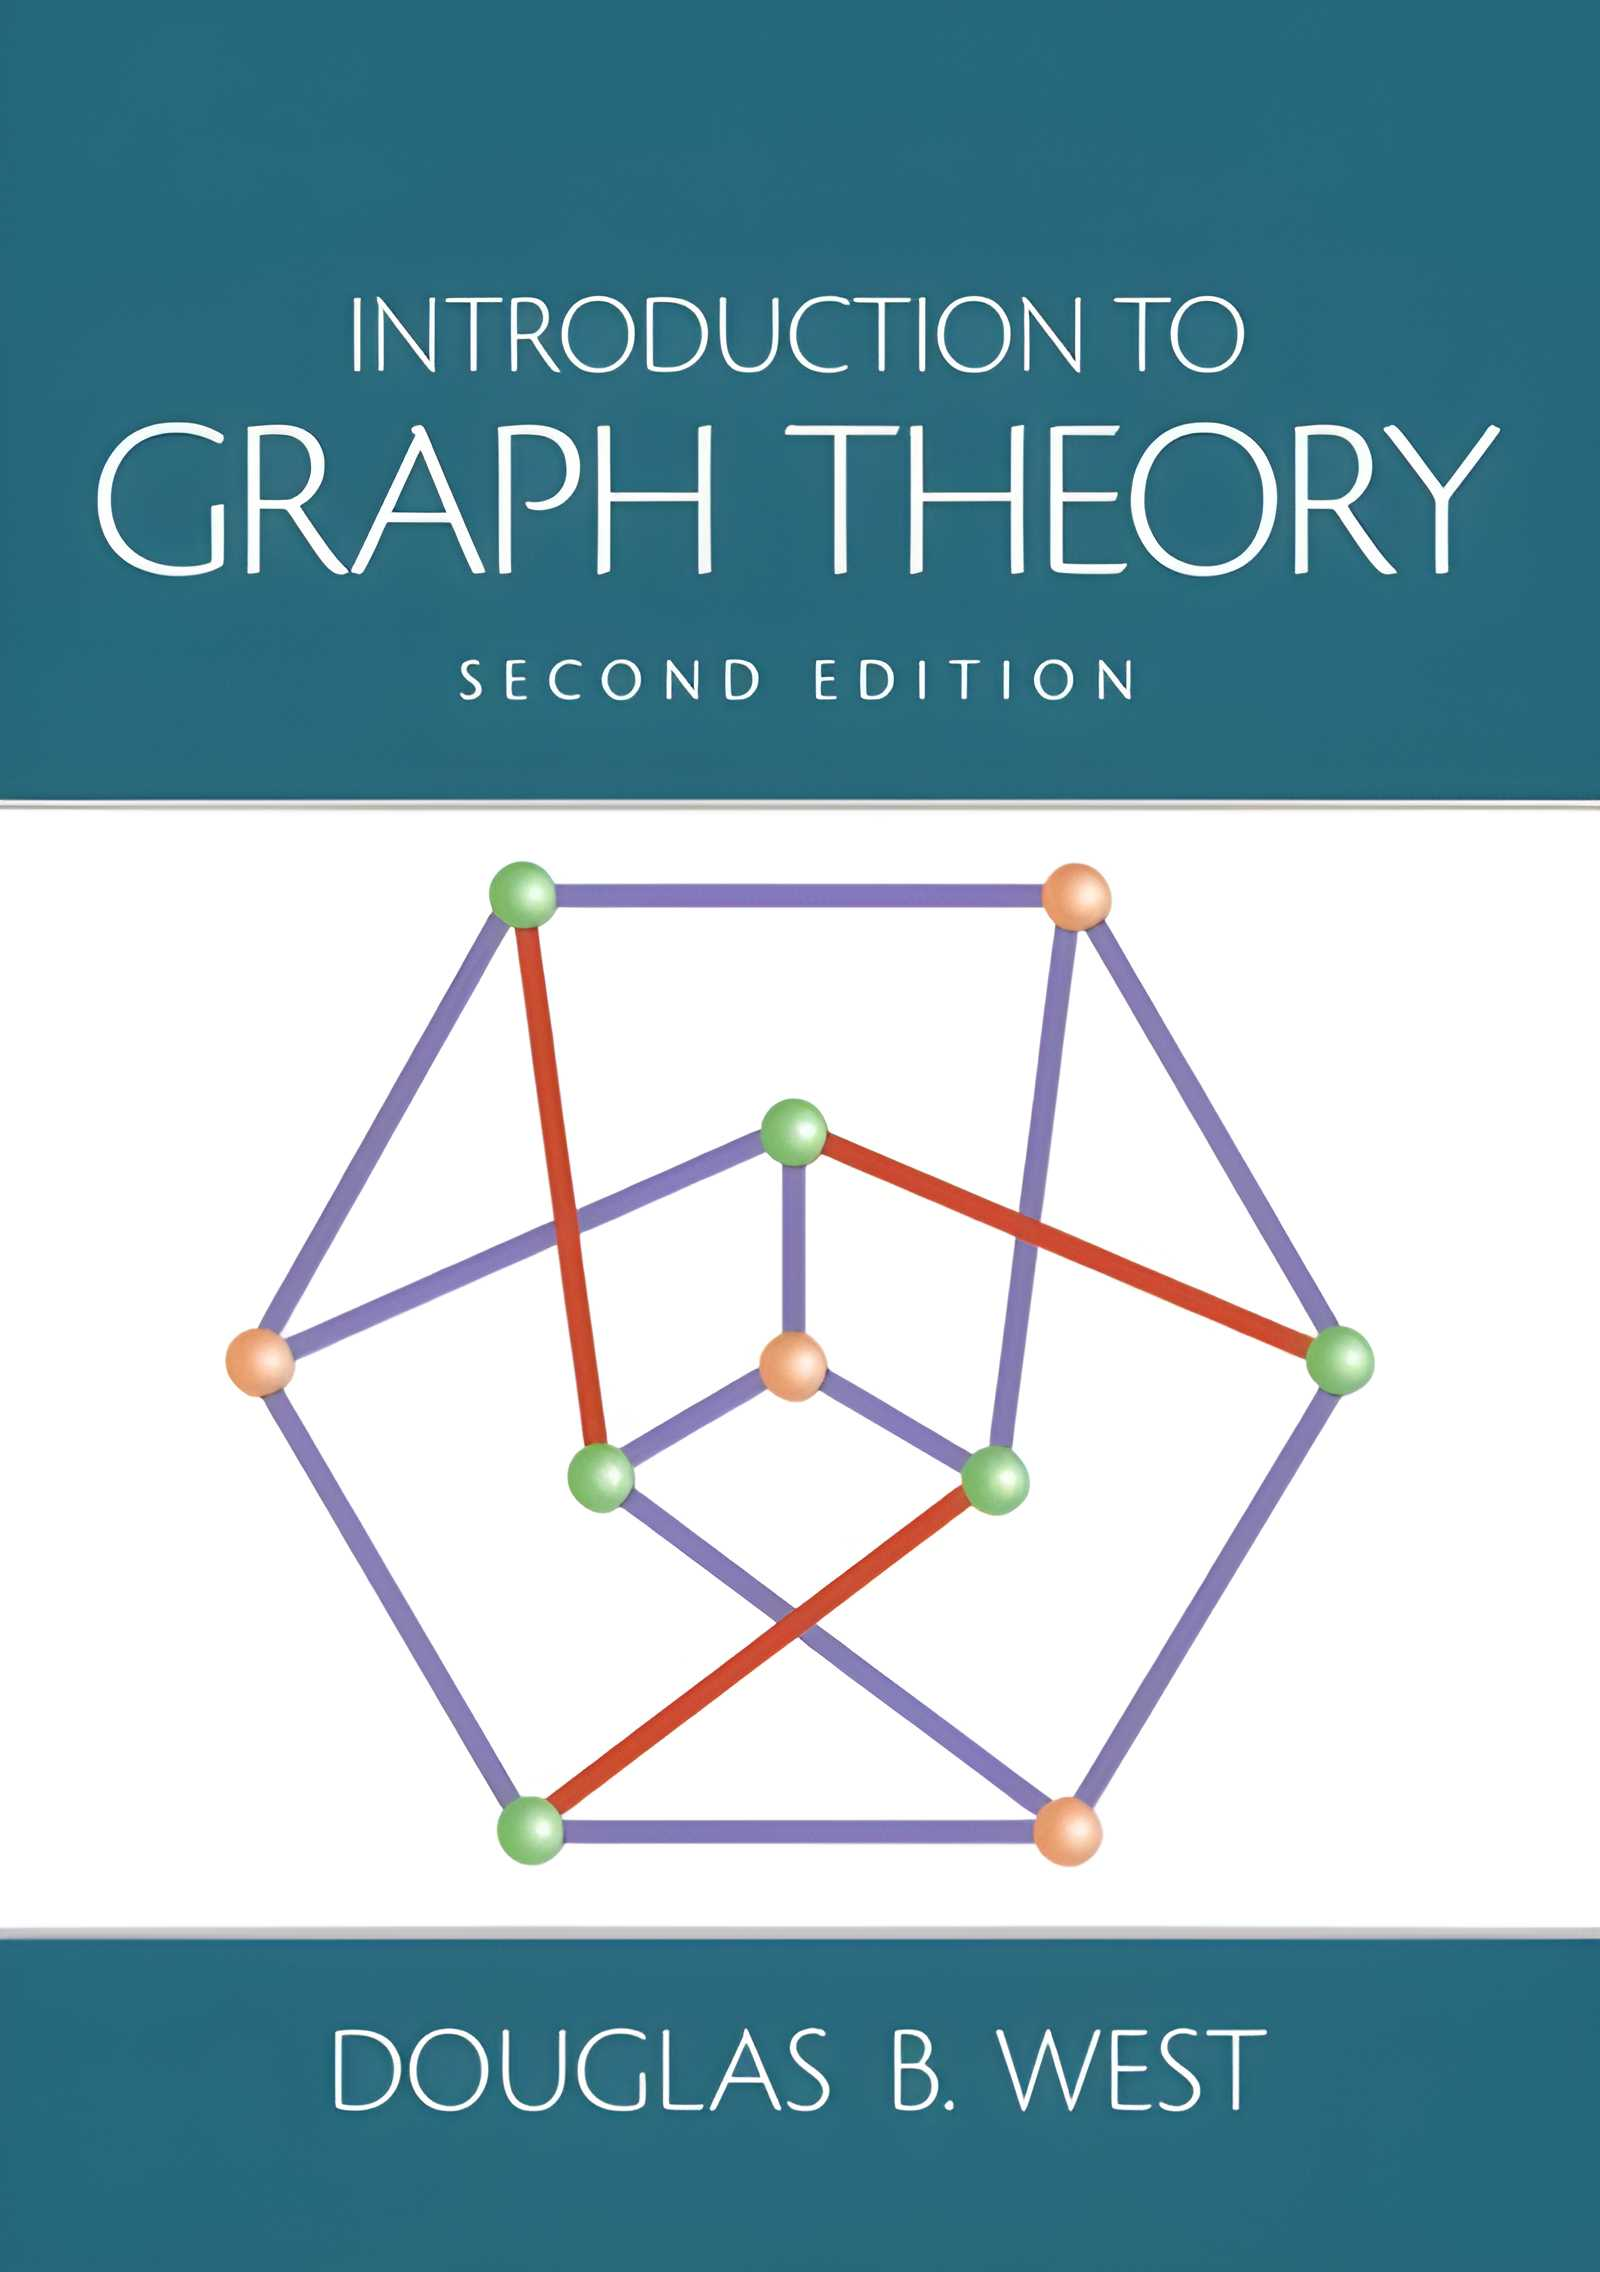
\includegraphics[width=\textwidth]{syllabus-textbook-front-cover_enlarged-by-upscalepics}
      \end{figure}
    \end{column}
  \end{columns}
\end{frame}

\begin{frame}{Schedule}
  \centering
  \begin{tabular}{llm{10cm}}
    \hline
    Week & Date & Content                                                                    \\ \hline
    1    & 2/23 & Syllabus                                                                   \\
    2    & 3/1  & Introduction \& Mathematical Background                                    \\
    3    & 3/8  & Fundamental Concept (1)                                                    \\
    4    & 3/15 & Fundamental Concept (2)                                                    \\
    5    & 3/22 & Fundamental Concept (3) \& \newline \textcolor{violet}{填寫Paper Survey 1表單} \\
    6    & 3/29 & Tree and Distance (1)                                                      \\
    7    & 4/5  & \textcolor{blue}{清明連假}                                                     \\
    8    & 4/12 & Tree and Distance (2)                                                      \\
    9    & 4/19 & \textcolor{red}{Midterm Exam} \& \textcolor{violet}{填寫Paper Survey 2表單}    \\ \hline
  \end{tabular}
\end{frame}

\begin{frame}{Schedule (Cont'd)}
  \centering
  \begin{tabular}{llm{7cm}}
    \hline
    Week & Date & Content                                                                   \\ \hline
    10   & 4/26 & Paper Presentation I (1)                                                  \\
    11   & 5/3  & Paper Presentation I (2)                                                  \\
    12   & 5/10 & Paper Presentation I (3) \& \newline \textcolor{violet}{程式作業(bonus)公告}    \\
    13   & 5/17 & Matching and Factors                                                      \\
    14   & 5/24 & Connectivity and Paths                                                    \\
    15   & 5/31 & Paper Presentation II (1)                                                 \\
    16   & 6/7  & Paper Presentation II (2) \& \newline \textcolor{violet}{程式作業(bonus)繳交期限} \\
    17   & 6/14 & Paper Presentation II (3)                                                 \\
    18   & 6/21 & \textcolor{red}{Final Exam}                                               \\ \hline
  \end{tabular}
\end{frame}

\begin{frame}{Two Paper Surveys}
  \begin{itemize}
    \item 1st time: Graph Theory (GT) on Digital Circuit/Software Design and Verification.
    \item 2nd time: GT on Machine Learning for Image/Video Enhancement/Processing.
  \end{itemize}
\end{frame}

\begin{frame}{Two Paper Presentations}
  \begin{enumerate}
    \item 2 persons per group.
    \item 1 paper per group per presentation.
    \item Presentation slides in PPTX or PDF with 20---50 pages.
    \item Time requirements (will be adjusted if needed):
      \begin{enumerate}
        \item 15---18 minutes for presentation.
        \item Additional 3---5 minutes for Q\&A.
      \end{enumerate}
    \item For fairness, all groups will have an identical due date.
    \item Apart from the slides, every group need to hand in a report in DOCX or PDF for more details, especially for the parts uncovered or hard to show in the presentation.
    \item You will fail with only translation. Otherwise, you will get more than 70 points, up to 99.
    \item Regard paper presentations as midterms.
  \end{enumerate}
\end{frame}

\begin{frame}{\textcolor{red}{Bonus} Program Exercise}
  \begin{enumerate}
    \item 1 person per group.
    \item No need to demonstrate it.
    \item Details will be announced later.
    \item \textcolor{red}{NO Delay and NO Plagiarism.}
    \item TA will review codes with code checking tool. With a similar piece of code among some people, all related individuals must take coding quizzes related to the program on site individually. If some ones quit, they get no bonus. If all pass, it's fine.
    \item It is allowed to reference code on the Internet without much similarity, for TAs can also access GitHub. With changes like variable names and coding style, it's fine.
  \end{enumerate}
\end{frame}

\begin{frame}{Evalution (評分方式)}
  \begin{enumerate}
    \item Close-booked exams \textcolor{red}{50\%} (more than 100 points for each)
      \begin{enumerate}
        \item Midterm 25\%
        \item Final Exam 25\%
      \end{enumerate}
    \item Two paper presentations \textcolor{red}{25\% per each}
    \item A \textcolor{red}{bonus} program exercise
    \item There is \textcolor{blue}{NO CHANCE TO MAKE AMENDMENTS} in the end of this semester (except everyone fails). Do NOT send email to me for this purpose.
  \end{enumerate}
\end{frame}

\begin{frame}{Rules to Avoid Unfair Evaluation}
  % TODO: add a floating "syllabus-you-cannot-pass_enlarged-by-upscalepics.png" in a corner
  \begin{enumerate}
    \item Anyone who \textcolor{red}{cheats in midterm or final exams} will be processed according to the \textcolor{blue}{college regulations}. No doubt, he/she will \textcolor{blue}{fail} in this class.
    \item Anyone who \textcolor{red}{plagiarizes other student's source code} will get \textcolor{blue}{zero point}, while the \textcolor{red}{original author} will get \textcolor{blue}{50\% off}.
    \item Anyone who plagiarizes source code from the Internet or students in previous years is also considered plagiarism. He/She will get zero point.
    \item Discussions in encouraged, but plagiarism is seriously prohibited. You must \textcolor{blue}{\textbf{write your own code}} after discussion.
  \end{enumerate}
\end{frame}

\begin{frame}{Acknowledgement}
  Content acknowledgement to Prof. Hsieh @ NCKU CSIE, Prof. Chang @ NTU MATH, and Prof. Fu @ NCTU MATH.
\end{frame}

\end{document}
